\begin{figure}[htbp]
			\centering
			\resizebox{\textwidth}{!}{%
				\begin{tikzpicture}[
					>=stealth,
					line cap=round,
					line join=round,
					]
					
					%============================================================
					% PANNELLO A — schema di carico (in alto a sinistra)
					%============================================================
					\begin{scope}[shift={(0,0)}]
						
						% aste
						\draw[line width=1.5pt] (2,1.4)--(4,1.4)--(6,1.4);
						\draw[line width=1pt] (0,0)--(4,0)--(8,0);
						\draw[line width=1pt] (0,0)--(2,1.4);
						\draw[line width=1pt] (2,1.4)--(4,0);
						\draw[line width=1pt] (4,0)--(4,1.4);
						\draw[line width=1pt] (4,0)--(6,1.4);
						\draw[line width=1pt] (6,1.4)--(8,0);
						
						% carico distribuito
						\draw (2,2.3)--(6,2.3);
						\foreach \x in {2, 2.67, 3.33, 4.00, 4.67, 5.33, 6.00}{
							\draw[->] (\x,2.3)--(\x,1.90);
						}
						\draw (2,1.90)--(6,1.90);
						\node[left, font=\small] at (2,2.10) {$q$};
						
						% vincolo cerniera A
						\draw[line width=1pt] (0,0)--(-0.4,-0.6)--(0.4,-0.6)--cycle;
						\draw[line width=0.8pt] (-0.50,-0.60)--(0.50,-0.60);
						\foreach \xi in {-0.40,-0.20,0.00,0.20}{
							\draw[thin] (\xi,-0.60)--(\xi-0.15,-0.85);
						}
						
						% vincolo carrello B
						\draw[line width=1pt] (8,0)--(7.60,-0.60)--(8.40,-0.60)--cycle;
						\draw[line width=0.8pt] (7.50,-0.60)--(8.50,-0.60);
						\draw[line width=0.8pt] (7.75,-0.69) circle(0.09);
						\draw[line width=0.8pt] (8.25,-0.69) circle(0.09);
						\draw[line width=0.8pt] (7.50,-0.78)--(8.50,-0.78);
						\foreach \xi in {7.50,7.70,7.90,8.10,8.30}{
							\draw[thin] (\xi,-0.78)--(\xi-0.15,-1.03);
						}
						
						% reazioni vincolari
						\draw[->, line width=1.5pt] (0,0)--(0,0.9);
						\node[left, font=\small] at (0,0.9) {$qd$};
						\draw[->, line width=1.5pt] (8,0)--(8,0.9);
						\node[right, font=\small] at (8,0.9) {$qd$};
						
						% nodi
						\foreach \x/\y in {0/0, 4/0, 8/0, 2/1.4, 4/1.4, 6/1.4}{
							\fill[white] (\x,\y) circle(3pt);
							\draw        (\x,\y) circle(3pt);
						}
						
						% etichette
						\node[above left,  font=\small] at (0,0)   {$A$};
						\node[below,       font=\small] at (4,0)   {$D$};
						\node[above right, font=\small] at (8,0)   {$B$};
						\node[above left,  font=\small] at (2,1.4) {$C$};
						\node[above left,  font=\small] at (4,1.4) {$E$};
						\node[above right, font=\small] at (6,1.4) {$F$};
						
						% etichetta pannello
						\node[font=\scriptsize] at (4,-1.3) {(a)};
						
					\end{scope}
					
					%============================================================
					% PANNELLO B — funzionamento strutturale (in alto a destra)
					%============================================================
					\begin{scope}[shift={(9.5,0)}]
						
						% aste compresse
						\draw[line width=2.5pt] (2,1.4)--(4,1.4)--(6,1.4);
						\draw[line width=2.5pt] (0,0)--(2,1.4);
						\draw[line width=2.5pt] (6,1.4)--(8,0);
						\draw[line width=2.5pt] (4,0)--(4,1.4);
						
						% aste tese
						\draw[line width=0.8pt] (0,0)--(4,0)--(8,0);
						\draw[line width=0.8pt] (4,0)--(6,1.4);
						\draw[line width=0.8pt] (2,1.4)--(4,0);
						
						% vincolo cerniera A
						\draw[line width=1pt] (0,0)--(-0.4,-0.6)--(0.4,-0.6)--cycle;
						\draw[line width=0.8pt] (-0.50,-0.60)--(0.50,-0.60);
						\foreach \xi in {-0.40,-0.20,0.00,0.20}{
							\draw[thin] (\xi,-0.60)--(\xi-0.15,-0.85);
						}
						
						% vincolo carrello B
						\draw[line width=1pt] (8,0)--(7.60,-0.60)--(8.40,-0.60)--cycle;
						\draw[line width=0.8pt] (7.50,-0.60)--(8.50,-0.60);
						\draw[line width=0.8pt] (7.75,-0.69) circle(0.09);
						\draw[line width=0.8pt] (8.25,-0.69) circle(0.09);
						\draw[line width=0.8pt] (7.50,-0.78)--(8.50,-0.78);
						\foreach \xi in {7.50,7.70,7.90,8.10,8.30}{
							\draw[thin] (\xi,-0.78)--(\xi-0.15,-1.03);
						}
						
						% nodi
						\foreach \x/\y in {0/0, 4/0, 8/0, 2/1.4, 4/1.4, 6/1.4}{
							\fill[white] (\x,\y) circle(3pt);
							\draw        (\x,\y) circle(3pt);
						}
						
						% etichette nodi
						\node[above left,  font=\small] at (0,0)   {$A$};
						\node[below,       font=\small] at (4,0)   {$D$};
						\node[above right, font=\small] at (8,0)   {$B$};
						\node[above left,  font=\small] at (2,1.4) {$C$};
						\node[above right, font=\small] at (4,1.4) {$E$};
						\node[above right, font=\small] at (6,1.4) {$F$};
						
						% legenda
						\draw[line width=2.5pt] (1.3,-0.8)--(2.3,-0.8);
						\node[right, font=\scriptsize] at (2.3,-0.8) {compressione};
						\draw[line width=0.8pt] (4.7,-0.8)--(5.7,-0.8);
						\node[right, font=\scriptsize] at (5.7,-0.8) {trazione};
						
						% etichetta pannello
						\node[font=\scriptsize] at (4,-1.7) {(b)};
						
					\end{scope}
					
					%============================================================
					% PANNELLO C — diagramma T(z) (in basso a sinistra)
					%============================================================
					\begin{scope}[shift={(0,-4.5)}]
						
						% diagramma T
						\fill[gray!20] (2,1.4)--(2,2.0)--(4,0.8)--(4,1.4)--cycle;
						\draw (2,2.0)--(4,0.8);
						\draw[dashed, thin] (2,1.4)--(4,1.4);
						\draw[thin] (2,1.4)--(2,2.0);
						\draw[thin] (4,1.4)--(4,0.8);
						
						\fill[gray!20] (4,1.4)--(4,2.0)--(6,0.8)--(6,1.4)--cycle;
						\draw (4,2.0)--(6,0.8);
						\draw[dashed, thin] (4,1.4)--(6,1.4);
						\draw[thin] (4,1.4)--(4,2.0);
						\draw[thin] (6,1.4)--(6,0.8);
						
						% quote
						\node[right, font=\small] at (2,2.0)   {$+\tfrac{qd}{2}$};
						\node[right, font=\small] at (4,0.9)   {$-\tfrac{qd}{2}$};
						\node[right, font=\small] at (4,2.0)   {$+\tfrac{qd}{2}$};
						\node[right, font=\small] at (5.8,0.7) {$-\tfrac{qd}{2}$};
						\node[right, font=\small] at (6.3,1.7) {$T(z)$};
						
						% travatura
						\draw[line width=1.5pt] (2,1.4)--(4,1.4)--(6,1.4);
						\draw[line width=1pt] (0,0)--(4,0)--(8,0);
						\draw[line width=1pt] (0,0)--(2,1.4);
						\draw[line width=1pt] (2,1.4)--(4,0);
						\draw[line width=1pt] (4,0)--(4,1.4);
						\draw[line width=1pt] (4,0)--(6,1.4);
						\draw[line width=1pt] (6,1.4)--(8,0);
						
						% vincolo cerniera A
						\draw[line width=1pt] (0,0)--(-0.4,-0.6)--(0.4,-0.6)--cycle;
						\draw[line width=0.8pt] (-0.50,-0.60)--(0.50,-0.60);
						\foreach \xi in {-0.40,-0.20,0.00,0.20}{
							\draw[thin] (\xi,-0.60)--(\xi-0.15,-0.85);
						}
						
						% vincolo carrello B
						\draw[line width=1pt] (8,0)--(7.60,-0.60)--(8.40,-0.60)--cycle;
						\draw[line width=0.8pt] (7.50,-0.60)--(8.50,-0.60);
						\draw[line width=0.8pt] (7.75,-0.69) circle(0.09);
						\draw[line width=0.8pt] (8.25,-0.69) circle(0.09);
						\draw[line width=0.8pt] (7.50,-0.78)--(8.50,-0.78);
						\foreach \xi in {7.50,7.70,7.90,8.10,8.30}{
							\draw[thin] (\xi,-0.78)--(\xi-0.15,-1.03);
						}
						
						% nodi
						\foreach \x/\y in {0/0, 4/0, 8/0, 2/1.4, 4/1.4, 6/1.4}{
							\fill[white] (\x,\y) circle(3pt);
							\draw        (\x,\y) circle(3pt);
						}
						
						% etichette nodi
						\node[above left,  font=\small] at (0,0)   {$A$};
						\node[below,       font=\small] at (4,0)   {$D$};
						\node[above right, font=\small] at (8,0)   {$B$};
						\node[above left,  font=\small] at (2,1.4) {$C$};
						\node[above left,  font=\small] at (4,1.4) {$E$};
						\node[above right, font=\small] at (6,1.4) {$F$};
						
						% etichetta pannello
						\node[font=\scriptsize] at (4,-1.3) {(c)};
						
					\end{scope}
					
					%============================================================
					% PANNELLO D — diagramma M(z) (in basso a destra)
					%============================================================
					\begin{scope}[shift={(9.5,-4.5)}]
						
						% diagramma M
						\fill[gray!20] (2,1.4) .. controls (3,0.8) .. (4,1.4)--cycle;
						\draw (2,1.4) .. controls (3,0.8) .. (4,1.4);
						\draw[dashed, thin] (2,1.4)--(4,1.4);
						\draw[thin] (3,1.4)--(3,0.8);
						\node[below, font=\small] at (3.5,1.1) {$\tfrac{qd^2}{8}$};
						
						\fill[gray!20] (4,1.4) .. controls (5,0.8) .. (6,1.4)--cycle;
						\draw (4,1.4) .. controls (5,0.8) .. (6,1.4);
						\draw[dashed, thin] (4,1.4)--(6,1.4);
						\draw[thin] (5,1.4)--(5,0.8);
						\node[below, font=\small] at (4.5,1.1) {$\tfrac{qd^2}{8}$};
						
						\node[right, font=\small] at (6.3,1.2) {$M(z)$};
						
						% travatura
						\draw[line width=1.5pt] (2,1.4)--(4,1.4)--(6,1.4);
						\draw[line width=1pt] (0,0)--(4,0)--(8,0);
						\draw[line width=1pt] (0,0)--(2,1.4);
						\draw[line width=1pt] (2,1.4)--(4,0);
						\draw[line width=1pt] (4,0)--(4,1.4);
						\draw[line width=1pt] (4,0)--(6,1.4);
						\draw[line width=1pt] (6,1.4)--(8,0);
						
						% vincolo cerniera A
						\draw[line width=1pt] (0,0)--(-0.4,-0.6)--(0.4,-0.6)--cycle;
						\draw[line width=0.8pt] (-0.50,-0.60)--(0.50,-0.60);
						\foreach \xi in {-0.40,-0.20,0.00,0.20}{
							\draw[thin] (\xi,-0.60)--(\xi-0.15,-0.85);
						}
						
						% vincolo carrello B
						\draw[line width=1pt] (8,0)--(7.60,-0.60)--(8.40,-0.60)--cycle;
						\draw[line width=0.8pt] (7.50,-0.60)--(8.50,-0.60);
						\draw[line width=0.8pt] (7.75,-0.69) circle(0.09);
						\draw[line width=0.8pt] (8.25,-0.69) circle(0.09);
						\draw[line width=0.8pt] (7.50,-0.78)--(8.50,-0.78);
						\foreach \xi in {7.50,7.70,7.90,8.10,8.30}{
							\draw[thin] (\xi,-0.78)--(\xi-0.15,-1.03);
						}
						
						% nodi
						\foreach \x/\y in {0/0, 4/0, 8/0, 2/1.4, 4/1.4, 6/1.4}{
							\fill[white] (\x,\y) circle(3pt);
							\draw        (\x,\y) circle(3pt);
						}
						
						% etichette nodi
						\node[above left,  font=\small] at (0,0)   {$A$};
						\node[below,       font=\small] at (4,0)   {$D$};
						\node[above right, font=\small] at (8,0)   {$B$};
						\node[above left,  font=\small] at (2,1.4) {$C$};
						\node[above left,  font=\small] at (4,1.4) {$E$};
						\node[above right, font=\small] at (6,1.4) {$F$};
						
						% etichetta pannello
						\node[font=\scriptsize] at (4,-1.3) {(d)};
						
					\end{scope}
					
			\end{tikzpicture}}
			\caption{Travatura a correnti paralleli con carico
				distribuito $q$ su $CE$ ed $EF$.
				\emph{(a)}: schema di carico.
				\emph{(b)}: funzionamento strutturale ---
				aste compresse a tratto spesso, aste tese
				a tratto sottile.
				\emph{(c)}: diagramma del taglio $T(z)$
				sulle aste $CE$ ed $EF$.
				\emph{(d)}: diagramma del momento $M(z)$
				sulle aste $CE$ ed $EF$.}
			\label{fig:assemblaggio_travatura}
		\end{figure}
